\begin{figure}[H]
  \centering
  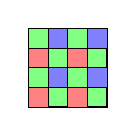
\begin{tikzpicture}
    \begin{scope}[shift={(0,0)}, local bounding box=sensorin]
      \filldraw[fill=green!50]   (0,0)     rectangle (1,1);
      \fill[fill=red!50]  (0,0)     rectangle (.25,.25);
      \fill[fill=red!50]  (.5,0)    rectangle (.75,.25);
      \fill[fill=red!50]  (.5,.5)   rectangle (.75,.75);
      \fill[fill=red!50]  (0,.5)    rectangle (.25,.75);
      \fill[fill=blue!50] (.25,.25) rectangle (.5,.5);
      \fill[fill=blue!50] (.75,.25) rectangle (1,.5);
      \fill[fill=blue!50] (.25,.75) rectangle (.5,1);
      \fill[fill=blue!50] (.75,.75) rectangle (1,1);
      \draw[step=.25,very thin] (0,0) grid (1,1);
    \end{scope}
  \end{tikzpicture}
  \caption{The Bayer CFA pattern}
  \label{fig:bayer}
\end{figure}
